\section{The 1-2 solar sector}
\label{sec:solar}

\subsection{The Sun interior and neutrino fluxes}

%A large amount of neutrinos arriving on Earth are produced by nuclear fusion reactions inside the Sun. 
The Sun is a star of the main sequence in the stable hydrogen fusion regime and it produces its energy by nuclear fusion reactions in its core described by the overall equation:
\begin{equation}
4p \rightarrow {}{^4}{\rm He} + 2 e^+ + 2 \nu_e
\label{eq:ppreac}
\end{equation}
After positron annihilation with electrons, the energy balance is equal to $E_s =26.73$ MeV per helium nucleus produced, including the mean energy of the neutrinos, amounting to approximately $E_\nu =$ 0.6 MeV. The total flux $\phi$ of solar neutrinos on Earth can be estimated from the solar constant (or solar irradiance) F = 1.36 kW/m$^2$  as
$\phi = \frac{2F}{E_s - E_\nu} = 6.5 \times 10^{10} {\rm cm^{-2} s^{-1}}$.

The resulting neutrino flux is due to several reaction chains contributing to the overall equation~(\ref{eq:ppreac}). The main reactions are shown in Table~\ref{tab:snuflux}, and the expected neutrino flux is shown in Fig.~\ref{fig:sol-spectra}. In addition to the pp chain, the catalytic CNO cycle involving carbon, nitrogen and oxygen nuclei, also takes place in the Sun. This cycle is dominant in more massive stars while in the Sun it only contributes about 2\% of the total energy production. 
The different neutrinos in the chain are usually referred by their parent particles  and, for the following of this discussion, it is important to notice that neutrinos from different reactions span different energy ranges. In particular the so-called $^{8}$B neutrinos are produced with energies up to 15 MeV and will be easier to observe in experiments with high energy thresholds, while $pp$ neutrinos, despite the larger flux, are more difficult to observe because of their low energy.
It must be noticed that these reactions have different dependences on the temperature and density and therefore the core regions where they take place differ. The $^8$B neutrinos are produced in the inner part of the core peaking at 0.05 of the solar radius. 


\begin{table}
\caption{Nuclear fusion reactions in the Sun and their neutrino fluxes (in units cm$^{-2}$ s$^{-1}$ times the factor in the fifth column) according to the SSM GS98-SFII and AGSS09-SFII~\cite{serenelli}, with relative uncertainties shown in the column labeled $\sigma$. The first five reactions are part of the pp chain, the last three reactions are part of the CNO cycle.}
\centering
\begin{tabular}{|c|c|c|c|c|c|c|}
  \hline
  Reaction & $E_{MAX}$ (MeV) & GS98 & AGSS09& exp. & $\sigma$ (\%) &name \\ 
  \hline
$ p + p \rightarrow {^2}H + e ^+ + \nu_e$ & 0.42 & 5.98  & 6.03   & $10^{10}$ & 0.6 &pp \\
$ p + e^- + p \rightarrow {^2}H  + \nu_e$ & 1.44 & 1.44  &1.47& $10^{9}$  & 1.2 &pep \\
$ {^7}Be + e^- \rightarrow {^7}Li + \nu_e$ & 0.86 & 5.00 & 4.56& $10^{9}$  & 7 &$ {^7}$Be \\
$ {^8}B \rightarrow {^8}Be + e ^+ + \nu_e$ & $\simeq$ 15 & 5.58  &4.59  &  $10^{6}$  & 14 &$ {^8}$B\\
$  {^3}He + p \rightarrow {^4}He + e ^+ + \nu_e$ & 18.77 & 8.04  &8.31 &$10^{3}$  & 30 &hep \\
$ {^{13}}N \rightarrow {^{13}}C + e ^+ + \nu_e$ & 1.2 & 2.96 &2.17    &$10^{8}$  &14  &$ {^{13}}$N\\
$ {^{15}}O \rightarrow {^{15}}N + e ^+ + \nu_e$ & 1.73 & 2.23 &1.56    &$10^{8}$  & 15& $ {^{15}}$O\\
$ {^{17}}F \rightarrow {^{17}}O + e ^+ + \nu_e$ & 1.74 & 5.52  &3.40   &$10^{6}$  & 16 &$ {^{17}}$F\\
  \hline
\end{tabular}
\label{tab:snuflux}
\end{table}

A Standard Solar Model (SSM)~\cite{bahcall89} is a model describing the Sun's interior structure and the thermonuclear reactions therein taking into account hydrostatic equilibrium, energy production and transport through radiation and convection, opacity and chemical composition. The chemical composition is expressed as the initial abundance of hydrogen $X$, helium $Y$ and elements heavier than lithium $Z$, with $X+Y+Z = 1$.
The SSM also needs to comply with various boundary conditions, like the observed luminosity and radius as well as the chemical composition at the surface. A SSM gives a prediction for the neutrino fluxes. 


%The main reactions and the corresponding neutrino fluxes are shown in  that is the dominant energy production mechanism for massive stars, is also present contributing about 1.6\% to the energy production.
%This cycle is dominant in massive stars.


Several SSM have been developed since the pioneering calculations by J. Bahcall in the 1960s, with slightly different assumptions. For example, two representative SSM models~\cite{serenelli}, GS98-SFII and AGSS09-SFII, differ in their assumptions for the abundance of heavier elements, the so called metallicity, which can only indirectly be evaluated from the solar atmosphere and from meteoritic abundances: $Z/X=0.023$ for GS98-SFII and $Z/X=0.018$ for AGSS09-SFII. These two models also predict slightly different fluxes of neutrinos, in particular the lower metallicity SSM AGSS09-SFII model predicts a 1\% cooler core which results in a 10\% lower flux of $^8$B and a smaller CNO produced neutrino flux.  

These models have been confronted with results from the helioseismology that studies the sound waves propagating inside the Sun, giving informations on the density and pressure profiles.
These data show good agreement for GS98-SFII but some discrepancy for AGSS09-SFII. 
This problem is known as the solar abundance or metallicity problem.


\begin{figure}[htbp]
\begin{minipage}[c]{.46\linewidth}
%\begin{minipage}[c]
   	      \includegraphics[width=0.9\linewidth]{figures/fig3_fluxes.pdf}
   \end{minipage} \hfill
   \begin{minipage}{.46\linewidth}
      \includegraphics[width=0.9\linewidth]{figures/fig4_oldexpts.pdf}
   \end{minipage}
    \caption{
Left: solar neutrino spectra and SSM uncertainties \cite{serenelli}.
Right: measurements of the solar neutrino fluxes by various experiments compared to the SSM prediction~\cite{serenelli}. Courtesy of Haxton et al.
}
\label{fig:sol-spectra}
\end{figure}


%\begin{figure}[htbp]
%\centering
%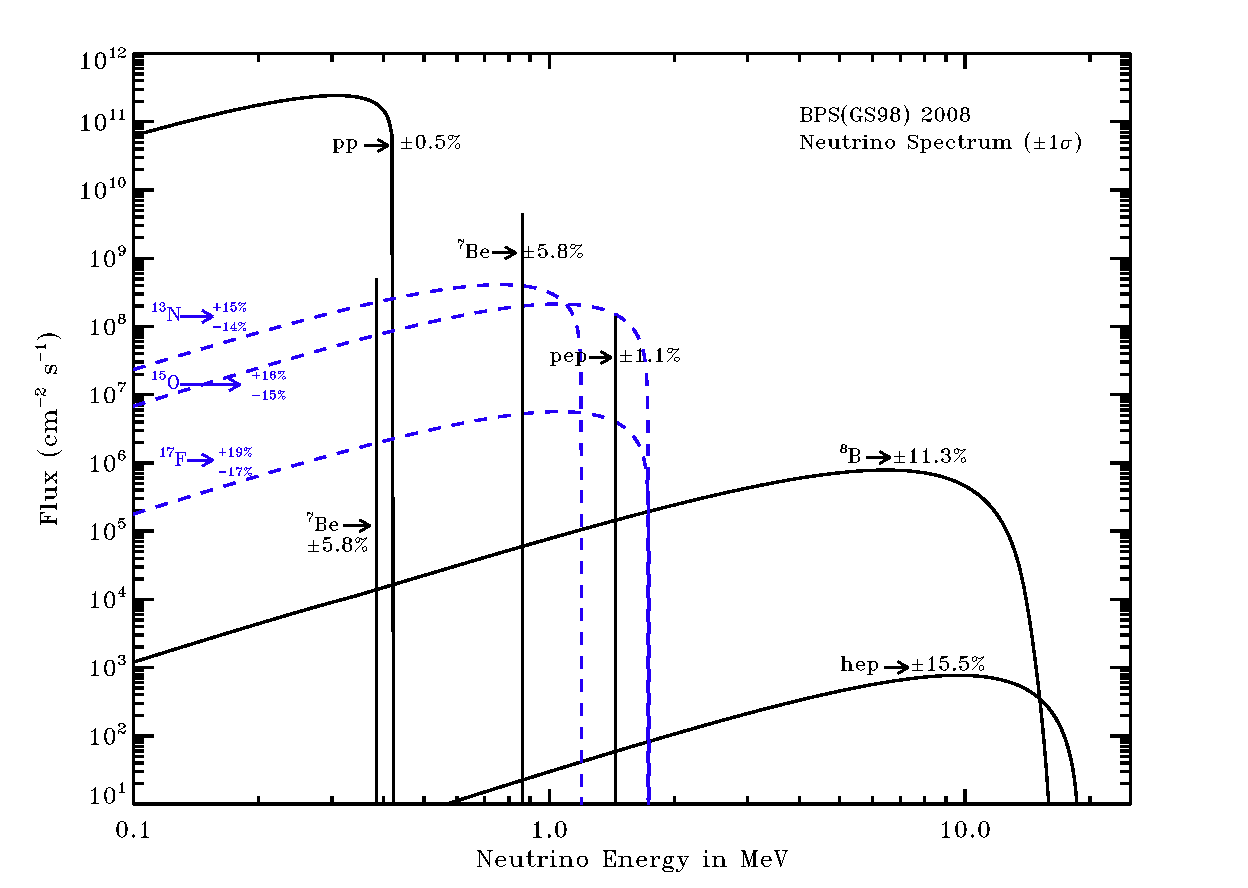
\includegraphics[width=0.6\linewidth]{figures/nu_spectrum1.pdf}
%  \caption{
%Solar neutrino spectra and SSM uncertainties \cite{serenellif}. 
%}
% \label{fig:sol-spectra}
% \end{figure}


\subsection{The early experiments}

The radiochemical detection of neutrinos using the reaction 
$\nu_e~^{37}Cl\rightarrow~^{37}Ar~e^-$ was first suggested by Bruno Pontecorvo in 1946~\cite{pontecorvo46}. This reaction has a threshold of 0.814 MeV and is therefore sensitive mainly to the $^8$B and $^7$Be solar neutrinos.

After previous experiments with this technique on surface, in 1965 Ray  Davis started  to construct a major experiment deep underground at Homestake (South Dakota), with 615~t of perchloroethylene (C$_2$Cl$_4$) that took data between 1968 and 2002.
The argon production rate induced by solar neutrino was 0.48 counts per day over a background of 0.09 counts per day due to the interactions initiated by highly energetic muons with nuclei (so called cosmogenics).
The $^{37}$Ar half-life of 35 days allows to expose the tank for a period of 60-70 days, followed by the efficient extraction of the produced argon by purging the liquid with helium.  
The isotope $^{37}$Ar decays by electron capture: 90 \% of these occur on the K-shell producing an average of 3.5 Auger electrons with 2.82 keV of total energy. Miniature gas proportional counters were developed to detect with high efficiency and purity these decays, achieving single-atom counting.
The efficiency of the whole extraction chain was calibrated injecting known quantities of other argon isotopes ($^{36}$Ar and $^{38}$Ar).  

The result of the Homestake chlorine experiment~\cite{cleveland} for the capture rate  is
\begin{equation}
(\sigma \phi)_{Cl} = 2.56 \pm 0.16 \pm 0.16 \: SNU
\end{equation}
where SNU is Solar Neutrino Units (a SNU equals 10$^{-36}$ captures/nucleus/second) while the prediction from the GS98-SFII solar model is $8.00 \pm 0.97$ SNU, that is the measured rate was about 30 \% of the predicted rate.  
Starting from the first result in 1968 this major deficit triggered a thirty years long debate, where many particle physicists were convinced that the SSM was not correct. Indeed the production rate of $ {^8}$B neutrinos depends critically on the temperature of the Sun core as T$^{22}$ and helioseismological data were not yet available at that time to confirm the validity of the SSM. 

\begin{table}
\caption{Solar neutrino detectors.}
\centering
\begin{tabular}{|c|c|c|c|c|c|}
  \hline
  Detector & Composition & Active mass & Threshold (MeV)  \\ 
  \hline
Homestake & C$_2$Cl$_4$ & 615t &  0.814 \\
Kamiokande & H$_2$O & 2.14kt &  7  \\
SAGE & Ga & 57t &  0.233 \\
GALLEX/GNO & Ga & 30.3t &  0.814  \\
Super-Kamiokande &  H$_2$O & 50kt &  3.5 \\
SNO & D$_2$O & 615 &  6\\
Borexino & C$_9$H$_{12}$ & 278t &  0.2  \\
  \hline
\end{tabular}

\label{tab:snudet}
\end{table}

It took more than twenty years before other radiochemical experiments could probe solar neutrinos~(Table~\ref{tab:snudet}). SAGE (1989-2007)~\cite{abdurashitov} in the Baksan Laboratory (Russia) and Gallex (1991-1997)~\cite{hampel}, followed by GNO (1998-2003)~\cite{altmann}, in the Gran Sasso Laboratory (Italy) used the reaction  $\nu_e  + {}^{71}{\rm Ga} \rightarrow {}^{71}{\rm Ge} + e^-$
that has a lower threshold, 0.233 MeV, and provides sensitivity to the $pp$ neutrinos, constituting the majority of the flux. 

While the details of these experiments, related to the chemical properties of gallium, is different from Homestake, they follow the same overall scheme of that experiment. They provided a confirmation of the solar neutrino deficit~\cite{abdurashitov,hampel,altmann,kaether}, although with a different reduction factor of approximately 50\% with respect the SSM prediction:
\begin{eqnarray}
(\sigma \phi)_{SAGE} & = & 65.4^{+3.1} _{-3.0} \; ^{+2.6} _{-2.8}  SNU \\
(\sigma \phi)_{GALLEX} & = & 73.4  ^{+6.1}_{-6.0} \; ^{+3.7} _{-4.1} SNU \\
(\sigma \phi)_{GNO} & = & 62.9  ^{+5.5} _{-5.3} \; ^{+2.5} _{-2.5} SNU 
\end{eqnarray}
to be compared with a predicted flux of 126.6 $\pm$ 4.2 SNU (GS98) (Fig.~\ref{fig:sol-spectra}).


\subsection{Real time experiments: Kamiokande, Super-Kamiokande, SNO, Borexino}

In 1987-1995 the 2.14 kt water Cherenkov experiment Kamiokande in Japan, in its phases II and III, provided a totally different measurement of the solar neutrinos flux. Neutrinos elastic scattering on electrons, mainly sensitive to electron neutrinos, could be detected with a threshold of 9 MeV, progressively reduced to 7 MeV.  
The water Cherenkov detection technique, also used later by the Super-Kamiokande and the SNO experiments, will be described in section~\ref{subsec:atmevidence}.   
Kamiokande was the first experiment to detect in real-time solar neutrinos. Since the scattered electron is emitted preferentially in the direction of the neutrino, it could verify their solar origin by correlating the electron momentum with the Sun direction. The combined result of Kamiokande~\cite{fukuda} is
\begin{equation}
\phi( ^8 B) = [2.80 \pm 0.19 (stat) \pm 0.33 (sys)] \times 10^6 {\rm cm^{-2} s^{-1}}
\end{equation}
providing another indication of a large suppression of the flux predicted by the solar model.

The 50kt water Cherenkov detector Super-Kamiokande, with a threshold of 7 MeV initially and today 3.5 MeV, started taking data in 1996 and confirmed the Kamiokande result with increased precision until its most recent update~\cite{abesk4}
\begin{equation}
\phi( ^8 B) = [2.308 \pm 0.020 (stat) ^{+0.040}_{-0.040} (sys)] \times 10^6 {\rm cm^{-2} s^{-1}}.
\end{equation} 

Super-Kamiokande is still running at present and it has recently observed for the first time a day-night effect for solar neutrinos~\cite{renshaw}. 
Let $r_D$ ($r_N$) be the day (night) event rate,
the day-night asymmetry $A_{DN}$ is defined as $A_{DN} = \frac{2 (r_D - r_N) }{r_D + r_N}$ and was measured to be
\begin{equation}
A_{DN} = (-3.2 \pm 1.1 (stat) \pm 0.5 (syst)) \%,
\end{equation} 
deviating from zero by 2.7 $\sigma$.
This is similar to $K_S^0$ regeneration for a beam of $K_L^0$ passing through a material. It is the first indication of Earth matter effects on neutrino propagation. 


%\begin{figure}[htbp]
%\centering
%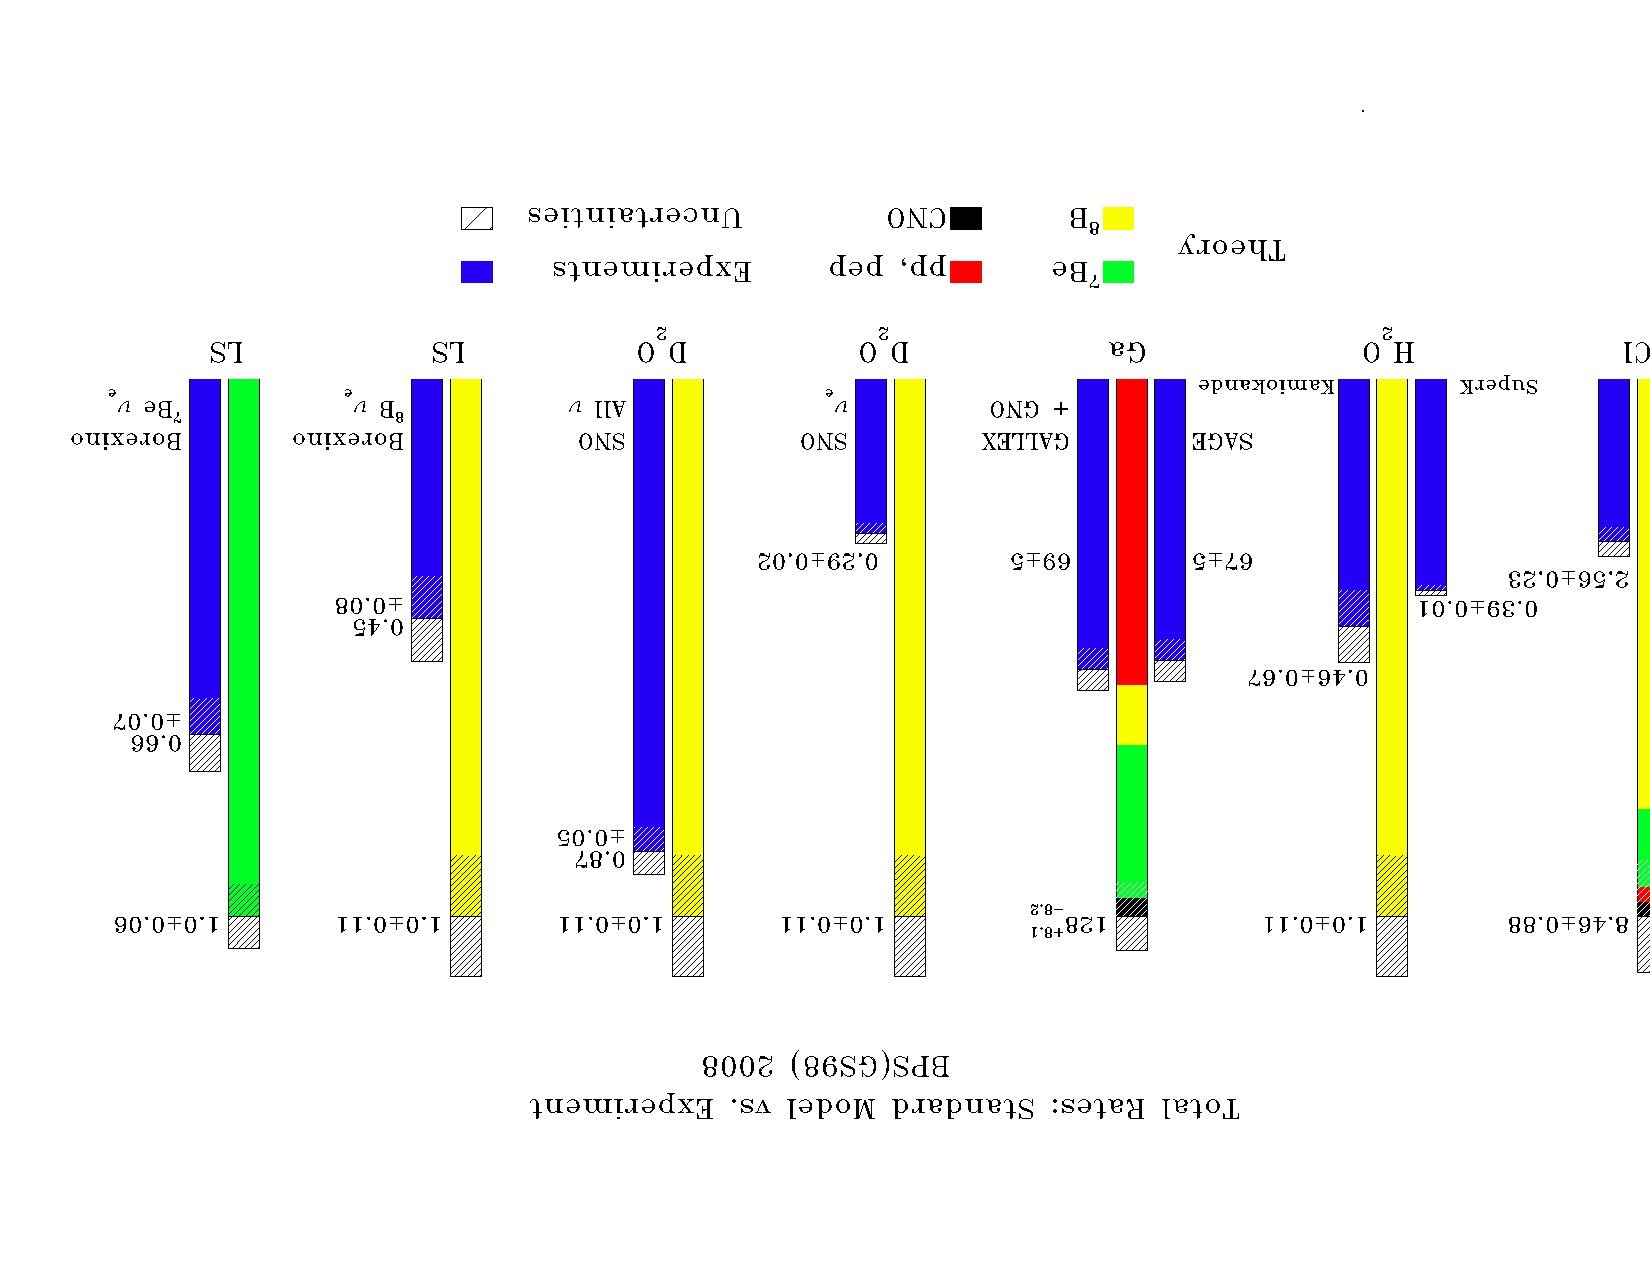
\includegraphics[angle=180,width=0.8\linewidth]{figures/theoryvsexpsnu1.pdf}
%  \caption{
%Measurements of the solar neutrino fluxes by various experiments compared to the SSM prediction~\cite{serenellif}.
%}
% \label{fig:sol-theoryexp}
% \end{figure}

The main limitations of the radiochemical and the water Cherenkov experiments is that they are only sensitive to charged current neutrino interactions with a \nue producing an electron in the final state. In this way it is not possible to distinguish between a deficit in the \nue flux due to a wrong SSM model prediction or a deficit due to neutrino oscillations.

The real breakthrough came from the Sudbury Neutrino Observatory (SNO, Canada), a Cherenkov detector 2 km below ground containing 1~kt of heavy water. 
With heavy water, three channels are available to probe the solar neutrino flux: 
\begin{itemize}
\item The charged current reaction for electron neutrinos $ \nu_e + d \rightarrow p + p + e^-$, where the produced electron carry off most of the neutrino energy allowing to constrain the neutrino spectrum;
\item The neutral current reaction $ \nu_x + d \rightarrow \nu_x +  p + n $ which allows to count all the neutrinos, independently of their flavour, above the threshold of 2.22 MeV; 
\item The electron scattering (ES) reaction $ \nu_x + e^- \rightarrow \nu_x + e^-$ also available in conventional water Cherenkov detectors, which is mainly sensitive to $ \nu_e$, as $\sigma_{ES}(\nu_e)\simeq 6 \; \sigma_{ES}(\nu_{\mu, \tau})$. 
\end{itemize}
SNO took data in three phases, distinguished by the technique used to detect the neutron produced in the neutral current dissociation of deuterium. Indeed, as the neutron is the only detectable particle in this reaction, this measurement is an experimental challenge and places severe requirements on the radiopurity of the whole apparatus. The different neutron detection techniques improved the sensitivity to the NC reactions. In the first phase neutron capture on deuterium was used. In the second phase, NaCl was dissolved in the water and neutrons were detected through the neutron capture on $^{35}$Cl followed by gamma emission. In the third phase neutron detectors containing $^3$He were inserted in the detector.
The electron kinetic energy threshold was 5 MeV, making the experiment sensitive to the ${}^8$B neutrinos. 
The results of all phases of the detector were in agreement and yielded a measurement of the total flux of solar neutrinos~\cite{aharmim}, irrespective of their flavour,
\begin{equation}
\phi_{NC} (\nu \; active ) = [5.25 \pm 0.16 (stat) ^{+0.11}
_{-0.13} (syst)] \times 10^6 {\rm cm^{-2} s^{-1}} 
\end{equation}
in agreement with the prediction of the solar models ($5.05 \times 10^6 {\rm cm^{-2} s^{-1}}$), and the flux of $\nu_e$
\begin{equation}
\phi_{CC} (\nu_e ) =  (0.301 \pm 0.033) \; \phi_{NC} (\nu \; active ).
\end{equation}
As we will discuss in section~\ref{subsec:solarinter} this is clearly an indication of flavour conversion of solar neutrinos. 

Finally another important experiment in the field of solar neutrino physics is the Borexino experiment that is running since 2007. Borexino is a 278~t liquid scintillator detector installed in the Gran Sasso Laboratory (Italy). 
It is capable of measuring low energy neutrinos with a threshold of 200 keV in real time, thanks to the high light yield of 10$^4$ photons per MeV which is much higher than in a Cherenkov detector and to the extreme levels of radiopurity reached inside the scintillator tank. 

Combining these two features Borexino was able to measure the flux of neutrinos from different reactions: the original goal of the experiment was the measurement of the $^7$Be neutrino flux that was measured to be $(3.10 \pm 0.15) \times 10^9 {\rm cm^{-2} s^{-1}}$ corresponding to the 62 \% of the GS98 SSM predicted flux~\cite{bellini}. It also provided the first determination of the pep flux 
$(1.6 \pm 0.3) \times 10^8 { \rm cm^{-2} s^{-1}}$ and a measurement of $^8$B neutrinos with a 3~MeV threshold. 
Finally they recently published the first real time observation of $pp$ neutrinos 
%measuring a flux, assuming LMA-MSW solution, of $(6.6\pm0.7)\times10^{10}{ \rm cm^{-2} s^{-1}}$ 
as well as the most stringent upper limit on the CNO neutrino flux. This is interesting since the flux of CNO neutrinos is sensitive to the assumption on the metallicity for the SSM.


\subsection{Confirmation with reactor neutrinos: KamLAND}

KamLAND is a 1~kt liquid scintillator experiment located in the former site of the Kamiokande detector in Japan. As described in more detail in section~\ref{subsec:reactorflux}, it is capable of detecting $\bar \nu_e$ emitted by nuclear reactors through the inverse beta decay reaction $\bar{\nu}_e \; p \rightarrow n \;  e^+$. KamLAND is surrounded by 55 Japanese nuclear reactors at an average distance of 150 km. In 2002, it reported first evidence for the disappearance  of $\bar \nu_e$. This measurement was very important for the interpretation of solar neutrino data as it showed for the first time an oscillatory behaviour as a function of L/E and it provided an independent and precise measurement of the oscillation parameters of interest.
In an updated report in 2013~\cite{Gando:2013nba}, they observed 2611 
events to be compared to $3564 \pm 145$ expected from reactor neutrinos in the case of no oscillation and  $364.1 \pm 30.5$ from background sources.
The KamLAND results are shown in Fig.~\ref{fig:sol-kam}. 

\begin{figure}[htbp]
\begin{minipage}[c]{.46\linewidth}
%\begin{minipage}[c]
   	      \includegraphics[width=0.9\linewidth]{figures/kamland_LE1.pdf}
   \end{minipage} \hfill
   \begin{minipage}{.46\linewidth}
      \includegraphics[width=0.9\linewidth]{figures/kamland_dmth1.pdf}
   \end{minipage}
    \caption{KamLAND experiment. The left plot shows the ratio of the background and geo-neutrino-subtracted $\bar{\nu}_e$
spectrum to the expectation for no-oscillation as a function of
L/E. The curve and histograms show the expectation for the best fit oscillation hypothesis. The right plot shows the allowed region for neutrino oscillation parameters from
KamLAND and solar neutrino experiments~\cite{Gando:2013nba}. Courtesy of the KamLAND collaboration.} 
 \label{fig:sol-kam}
\end{figure}


\subsection{Interpretation of the measurements and discussion}
\label{subsec:solarinter}

The first measurement of a deficit of the solar neutrino flux left open several interpretations. While early on Pontecorvo made the hypothesis of neutrino oscillations~\cite{Pontecorvo:1967fh}, modest changes to the Sun core temperature could also be invoked to explain the apparent deficit. 
The situation changed with the new measurements by the gallium experiments, as it was clear that the suppression factor depended on the neutrino energy. The SNO results were the first measurement of the total solar neutrino flux and were also the first solid proof of flavour conversion as the explanation of the solar neutrino puzzle. 

Nevertheless, several different solutions were possible in the early days in terms of masses and mixing. The KamLAND result pinpointed one of them, the so-called Large Mixing Angle (LMA) solution which was already favoured by SNO data. Indeed, the results of KamLAND can be understood in terms of a simple two neutrino mixing formula $ P(\bar{\nu}_e \rightarrow \bar{\nu}_e ) = 1 - \sin^2 2 \theta_{12} \sin^2 (\frac{\Delta m^2_{21} L}{4 E}) $, neglecting matter effects and effects related to $\theta_{13}$ (cf. Eq.~(\ref{eq:nuereactor})). 

As we will see later, the value of $\Delta m^2_{31}$ is much larger than $\Delta m^2_{21}$ and induces rapid oscillations that are averaged out given the large $L/E$ and the energy resolution of that experiment. The $L/E$ pattern is prominent in the KamLAND data and beautifully confirms neutrino oscillations as the origin of the observed deficit (Fig.~\ref{fig:sol-kam}). The measurement of KamLAND, when combined with solar neutrino experiments, allows to determine $\Delta m^2_{21} = (7.53 \pm 0.18) \times 10^{-5} eV^2$ and $\tan^2 \theta_{12} = 0.44 \pm 0.03$. The agreement between solar neutrino experiments and KamLAND is good, as shown in Fig.~\ref{fig:sol-kam}.

The explanation of the deficit observed by the solar neutrino experiments involves flavour transitions of a different kind. As explained in section~\ref{subsec:varying}, electron neutrinos are produced in the core of the Sun in a medium of high density. 
In the center of the Sun, the density $n(r=0)$ corresponds to the resonant density $ n_{res}= \frac{\Delta m^2_{21} \cos 2 \theta_{12}}{ 2 \sqrt{2}G_F E}$ for E = 1.9 MeV. For energies much higher than this value
%If the condition $n(r) > n_{res}= \frac{\Delta m^2_{21} \cos 2 \theta_{12}}{ 2 \sqrt{2}G_F E}$ is satisfied, corresponding to energies above 3.3 MeV for pp, 2.2 MeV for $^7$Be and 1.8 MeV for $^8$B neutrinos, 
neutrinos are produced as the $ \nu^m_2$ matter eigenstates of the Hamiltonian and in its adiabatic evolution exits the Sun as $\nu_2$. The probability to observe them as $\nu_e$ is then $\sin^2 \theta_{12} \sim 0.3$. 

For neutrinos produced with energies much below this threshold, matter effect can be neglected and they undergo vacuum oscillations. The suppression factor observed on Earth is then the result of the averaging of many oscillation periods    
$ P({\nu}_e \rightarrow {\nu}_e ) = 1 - \frac{1}{2} \sin^2 2 \theta_{12} \sim 0.58$. 
This leads to a characteristic "bath tub" shape for the neutrino survival probability (Fig.~\ref{fig:sol-bor}). The adiabatic flavour conversion dominates for $^8$B neutrinos, while pp are in the average vacuum oscillation region. 
%The measurement of pep neutrinos would be interesting as they are in the transition region.
This interpretation fits with all the solar neutrino data. 

The future of this field is twofold. The solar neutrino experiments will try to measure the CNO neutrinos as this is both interesting {\it per se} (the original motivation to study the solar neutrinos was in fact to understand how the Sun shines) and it will shed some light on the solar abundance problem. This will be attempted by Borexino and SNO+~\cite{snoplus}, with liquid scintillator instead of the heavy water in the inner vessel. 

The upturn of the solar neutrino survival probability, that is the transition from the MSW to the vacuum oscillation regime, in the few MeV region, is predicted by the MSW model, however it has not yet been observed. 
Experimentally this is very difficult as it requires to lower the threshold and to have a good control of the backgrounds. The failure so far to observe this upturn is also related to the mild tension reported by global fits of neutrino properties between the $\Delta m^2_{21}$ measured by KamLAND and the measurement using solar neutrino data~\cite{nufit}. Precision measurements of the solar neutrino flux are also a powerful probe of new physics scenarios.
 
On the other hand the long baseline reactor experiment JUNO, using the same technique as KamLAND, with 20~kt liquid scintillator will dramatically improve the precision, below the percent level, on the solar oscillation parameters  $\Delta m^2_{21}$ and $\theta_{12}$.

\begin{figure}[htbp]
\centering
\includegraphics[width=0.6\linewidth]{figures/pee.pdf}
  \caption{
  Solar neutrino survival probability as a function of the energy with the Borexino results \cite{derbin2016}. The gray band correspond to the $\pm1\sigma$ prediction of the MSW-LMA solution. Courtesy of the Borexino collaboration.
}
 \label{fig:sol-bor}
 \end{figure}
